\documentclass[10pt,xcolor=pdflatex,dvipsnames,table]{beamer}
\usepackage{newcent}
\usepackage[utf8]{inputenc}
\usepackage[czech]{babel}
\usepackage{hyperref}
\usepackage{amsthm}
\usepackage{amssymb}
\usepackage{amsmath}
\usepackage{array}
\usepackage{stmaryrd}
\usepackage{graphicx}
\usepackage{tabularx}
\usepackage{listings}
\usepackage{fancyvrb}
\usepackage{minted}
\usepackage{multicol}
%\usepackage{packages/beamerthemeFIT}

\makeatletter
  \def\beamer@calltheme#1#2#3{%
    \def\beamer@themelist{#2}
    \@for\beamer@themename:=\beamer@themelist\do
    {\usepackage[{#1}]{\beamer@themelocation/#3\beamer@themename}}}

  \def\usefolder#1{
    \def\beamer@themelocation{#1}
  }
  \def\beamer@themelocation{}

\usefolder{packages}
\usetheme{FIT}



\title[OpenGL]{PGR - Vertex Shader transformace}

\author[]{Tomáš Milet}

\institute[]{Brno University of Technology, Faculty of Information Technology\\
Bo\v{z}et\v{e}chova 1/2. 612 66 Brno - Kr\'alovo Pole\\
imilet@fit.vutbr.cz}

\date{\today}

\begin{document}

\frame[plain]{\titlepage}

\setbeamercolor{background canvas}{bg=fitblue}
\begin{frame}
\frametitle{Geometry Shader}
\begin{center}
\Huge {\color{white}Geometry Shader}
\end{center}
\end{frame}
\setbeamercolor{background canvas}{bg=white}

\begin{frame}[fragile]
\frametitle{Geometry shader}
  \scriptsize
	\begin{itemize}
    \item Geometry shader is located between rasterisation and vertex shader (after tessellation).
	  \item It processes primitives - It can access all atributes of all primitive vertices.
    \item It can generate or modify geometry (a point to polygon).
    \item It can be used for various effect (shadows, particle systems, debug draws).
	  \item Geometry Instancing.
	  \item Transform feedback.
	\end{itemize}
	\begin{itemize}
	  \item Geometry shader se nachází za vertex shaderem (za teselací).
	  \item Pracuje po primitivech - má přítup ke všem atributům všech vrcholů vstupního primitiva
	  \item Umožňuje generování geometrie a její úpravu.
	  \item Transformaci bodu na polygon. 
	  \item Používá se pro různé efekty (např. stíny (pomocí stínových těles)).
	  \item Další využití může být v částicových systémech.
	  \item Geometry Instancing.
	  \item Transform feedback.
	\end{itemize}
\end{frame}

\begin{frame}[fragile]
\frametitle{Geometry shader - inputs/outputs}
  \scriptsize
	\begin{itemize}
  \item Type of input primitive has to be specified inside geometry shader.
	\item V Geometry shaderu je nutné specifikovat typ vstupního primitiva.
	{\scriptsize
\begin{minted}[bgcolor=bg]{packages/graphics.py:GLShaderLexer -x}
layout(points,invocations=N)in;//vstupni primitivum bude bod
//points, lines, lines_adjacency, triangles, triangles_adjacency
//invocations - kolikrat bude GS spusten na jedno primitivum
	\end{minted}
	}
	\item Type of output primitive has to be also specified as well as maximal number of vertices.
	\item Také je nutné definovat výstupní primitivum a maximální počet výstupních vertexů.
	{\scriptsize
\begin{minted}[bgcolor=bg]{packages/graphics.py:GLShaderLexer -x}
layout(triangle_strip,max_vertices=4)out;//vystup je sekvence troj.
//points, line_strip, triangle_strip
	\end{minted}
	}
	\end{itemize}
\end{frame}

\begin{frame}[fragile]
\frametitle{Geometry shader - a point to square}
	\begin{figure}[h]
		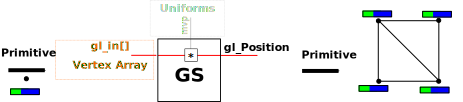
\includegraphics[width=9cm,keepaspectratio]{pics/geometryShader/gs.pdf}
	\end{figure}
  \scriptsize

	{\scriptsize
\begin{minted}[bgcolor=bg]{packages/graphics.py:GLShaderLexer -x}
#version 430

layout(points)in;
layout(triangle_strip,max_vertices=4)out;

void main(){
  gl_Position=mvp*(gl_in[0].gl_Position+vec4(-1,-1,0,0));
  EmitVertex();
  gl_Position=mvp*(gl_in[0].gl_Position+vec4(-1,+1,0,0));
  EmitVertex();
  gl_Position=mvp*(gl_in[0].gl_Position+vec4(+1,-1,0,0));
  EmitVertex();
  gl_Position=mvp*(gl_in[0].gl_Position+vec4(+1,+1,0,0));
  EmitVertex();
  EndPrimitive();
}
	\end{minted}
	}
\end{frame}

\begin{frame}[fragile]
\frametitle{Geometry shader - fullscreen quad}
	{\scriptsize
\begin{minted}[bgcolor=bg]{packages/graphics.py:GLShaderLexer -x}
#version 430
layout(points)in;
layout(triangle_strip,max_vertices=4)out;
void main(){
  gl_Position=vec4(-1,-1,0,1);EmitVertex();
  gl_Position=vec4(-1,+1,0,1);EmitVertex();
  gl_Position=vec4(+1,-1,0,1);EmitVertex();
  gl_Position=vec4(+1,+1,0,1);EmitVertex();
  EndPrimitive();
}
	\end{minted}
	}
	{\scriptsize
\begin{minted}[bgcolor=bg]{packages/c_cpp.py:CppLexer -x}
glCreateVertexArrays(1,&emptyVAO);
//...
glBindVertexArray(emptyVAO);//empty VAO
glDrawArrays(GL_POINTS,0,1);
glBindVertexArray(0);
	\end{minted}
	}
\end{frame}

\begin{frame}[fragile]
\frametitle{shadow volumes - zfail}
  \begin{figure}[h]
    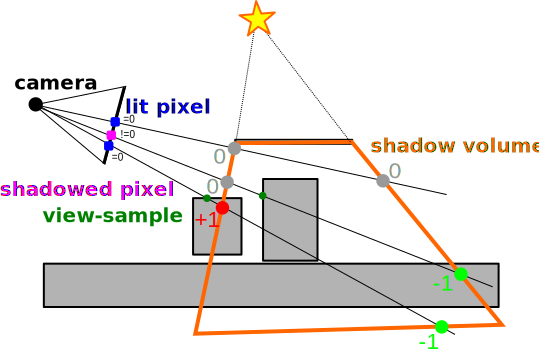
\includegraphics[width=11cm,keepaspectratio]{pics/geometryShader/shadowvolume.pdf}
  \end{figure}
\end{frame}

\begin{frame}[fragile]
\frametitle{Geometry shader - shadow volumes}
  \begin{columns}[T]
    \begin{column}{.44\textwidth}
	    {\tiny
\begin{minted}[bgcolor=bg]{packages/graphics.py:GLShaderLexer -x}
#version 330
layout(triangles)in;
layout(triangle_strip,max_vertices=10)out;
uniform mat4 MVP,M;//matice
uniform vec4 LightPosition;//pozice svetla
void main(){
  vec4 LP=M*LightPosition;
  vec4 p[6];
  p[0]=gl_in[0].gl_Position;//triangle points
  p[1]=gl_in[1].gl_Position;
  p[2]=gl_in[2].gl_Position;
  p[3]=vec4(gl_in[0].gl_Position.xyz*LP.w-LP.xyz,0);//in infinity
  p[4]=vec4(gl_in[1].gl_Position.xyz*LP.w-LP.xyz,0);
  p[5]=vec4(gl_in[2].gl_Position.xyz*LP.w-LP.xyz,0);
  vec3 N=normalize(cross((p[1]-p[0]).xyz,(p[2]-p[0]).xyz));
  float Distance=dot(N,LP.xyz)-dot(N,p[0].xyz);
  if(Distance<=0){//otocime volume vnitrkem ven
    vec4 c=p[0];p[0]=p[1];p[1]=c;
    c=p[3];p[3]=p[4];p[4]=c;
  }
  gl_Position=MVP*p[0];EmitVertex();
  gl_Position=MVP*p[1];EmitVertex();
  gl_Position=MVP*p[3];EmitVertex();
  gl_Position=MVP*p[4];EmitVertex();
  gl_Position=MVP*p[5];EmitVertex();
  gl_Position=MVP*p[1];EmitVertex();
  gl_Position=MVP*p[2];EmitVertex();
  gl_Position=MVP*p[0];EmitVertex();
  gl_Position=MVP*p[5];EmitVertex();
  gl_Position=MVP*p[3];EmitVertex();
  EndPrimitive();
}
    	\end{minted}
   	}
    \end{column}
    \begin{column}{.48\textwidth}
	    \begin{figure}[h]
    		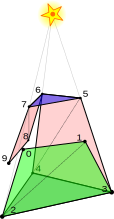
\includegraphics[width=3cm,keepaspectratio]{pics/geometryShader/PerTriangle.pdf}
    	\end{figure}
    \end{column}
  \end{columns}

\end{frame}


\setbeamercolor{background canvas}{bg=fitblue}
\begin{frame}
\frametitle{Transform feedback}
\begin{center}
\Huge {\color{white}Transform feedback}
\end{center}
\end{frame}
\setbeamercolor{background canvas}{bg=white}

\begin{frame}
\frametitle{Transform feedback}
	\begin{itemize}
	\item Zápis primitiv do bufferu
	\item Hlavně v Geometry Shaderu
	\item Streams (kreslení i zápis o bufferu)
	\end{itemize}
	\begin{figure}[h]
	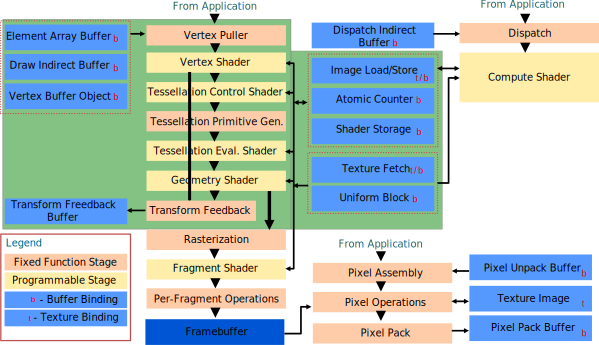
\includegraphics[width=10cm,keepaspectratio]{pics/transformFeedback/tf_pipeline}
	\end{figure}
\end{frame}

\begin{frame}
\frametitle{Transform feedback}
	\begin{figure}[h]
	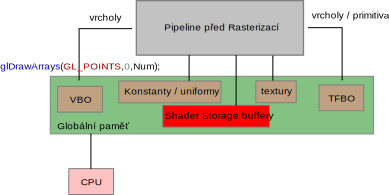
\includegraphics[width=10cm,keepaspectratio]{pics/transformFeedback/tf_mem}
	\end{figure}
\end{frame}

\begin{frame}[fragile]
\frametitle{Transform feedback - příklad}
	{\scriptsize
	\begin{minted}[frame=lines]{c++}
	const char*Vayrings[]={"Out1", "Out2"};
	glTransformFeedbackVaryings(Program,2,Varyings,GL_SEPARATE_ATTRIBS);
	glLinkProgram(Program);

	//...

	glBindBufferBase(GL_TRANSFORM_FEEDBACK_BUFFER,0,Buffer1);
	glBindBufferBase(GL_TRANSFORM_FEEDBACK_BUFFER,1,Buffer2);
	
	glEnable(GL_RASTERIZER_DISCARD);//nebudeme rasterizovat
	//...
	glBeginTransformFeedback(GL_TRIANGLES);
	glDrawArrays(...);
	glEndTransformFeedback();
	\end{minted}
	}
\end{frame}

\begin{frame}[fragile]
\frametitle{Transform Feedback - Inicializace}
	Slinkovat program s nastavenými výstupními proměnnými v shaderu.
	c++:
	{\scriptsize
	\begin{minted}[frame=lines]{cpp}
	//seznam promennych v shaderu, ktere se budou pomoci TF zapisovat do bufferu
	const char*ResetVaryings[]={"vPosition","vVelocity","vMass"};
	//nastavime seznam a nastavime prokladany zapis
	glTransformFeedbackVaryings(ResetProgram,3,ResetVaryings,GL_INTERLEAVED_ATTRIBS);
	//znovu slinkujeme program
	glLinkProgram(ResetProgram);
	\end{minted}
	}
	glsl:
	{\scriptsize
	\begin{minted}[frame=lines]{glsl}
	#version 330

	layout(location=0)out vec2  vPosition;//pozice castice
	layout(location=1)out vec2  vVelocity;//rychlost castice
	layout(location=2)out float vMass;//hmotnost castice
	//...
	void main(){
	  vPosition = vec2(0);//pozice do prostred
	  vVelocity = vec2(cos(VelAngle),sin(VelAngle))*VelSize;//rychlost jako vektor
	  vMass     = Noise(MassSeed+uint(gl_VertexID),MinMass,MaxMass);//hmotnost
	}
	\end{minted}
	}
\end{frame}


\setbeamercolor{background canvas}{bg=fitblue}
\begin{frame}
\frametitle{Teselace}
\begin{center}
\Huge {\color{white}Teselace}
\end{center}
\end{frame}
\setbeamercolor{background canvas}{bg=white}

\begin{frame}[fragile]
\frametitle{Teselace}
	\begin{itemize}
	\item Teselace je rozřezání jednoho primitiva na více spojených.
	\item Může se použít pro zjemnění geometrie
	\item Nachází se za vertex shaderem a před geometry shaderem.
	\item Složená ze 3 částí:
	\begin{itemize}
	\item Control Shader
	\item Generování primitiv/Teselace
	\item Evaluation Shader
	\end{itemize}
	\item Nový typ primitiva \textcolor{red}{GL\_PATCHES}
	\end{itemize}
  {\scriptsize
	\begin{minted}[frame=lines]{c++}
glPatchParameteri(GL_PATCH_VERTICES,10);//nastavi pocet vrcholu patche - 10
glDrawArrays(GL_PATCHES,0,100);//vykresli 10 patchu po 10 vrcholech
	\end{minted}
  }
	\begin{figure}[h]
	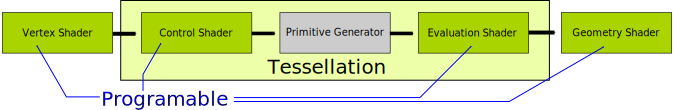
\includegraphics[width=10cm,keepaspectratio]{pics/tessellation/tess_pipeline.pdf}
	\end{figure}
\end{frame}

\begin{frame}
\frametitle{Control Shader}
	\begin{itemize}
	\item Řídí stupěň teselace
	\item Počítá kontrolní body
	\item Je spouštěn tolikrát, kolik je vertexů ve výstupním primitivu
	\item Číslo spuštění uloženo v \textcolor{OliveGreen}{gl\_InvocationID}
	\item \textcolor{OliveGreen}{barrier}()
	\end{itemize}
	\begin{figure}[h]
	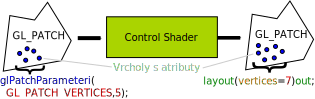
\includegraphics[width=10cm,keepaspectratio]{pics/tessellation/tess_control.pdf}
	\end{figure}
\end{frame}

\begin{frame}
    \frametitle{Parametry}

    
\includegraphics[width=\textwidth]{pics/tessellation/tess.pdf}

    \begin{itemize}
				\item \textcolor{OliveGreen}{layout}
					(\{\textcolor{orange}{isolines},\textcolor{orange}{triangles},\textcolor{orange}{quads}\})
					\textcolor{OliveGreen}{in};
				\item \textcolor{OliveGreen}{gl\_TessLevelOuter}[4],\textcolor{OliveGreen}{gl\_TessLevelInner}[2]
    \end{itemize}
\end{frame}

\begin{frame}[fragile]
\frametitle{Control Shader - příklad}
	{\scriptsize
	\begin{minted}[frame=lines]{glsl}
#version 430

// pocet vertexu ve vystupni primitivu
// pocet spusteni control shaderu
layout(vertices=3)out;

uniform vec2 TessLevelInner;//vnitrni deleni
uniform vec4 TessLevelOuter;//deleni hran

void main(){
  //velikost gl_in zavisi na GL_PATCH_VERTICES
  //velikost gl_out zavisi na layout(vertices=n)out;
  gl_out[gl_InvocationID].gl_Position=gl_in[gl_InvocationID].gl_Position;
  if(gl_InvocationID==0){
    gl_TessLevelOuter[0]=TessLevelOuter[0];
    gl_TessLevelOuter[1]=TessLevelOuter[1];
    gl_TessLevelOuter[2]=TessLevelOuter[2];
    gl_TessLevelOuter[3]=TessLevelOuter[3];
    gl_TessLevelInner[0]=TessLevelInner[0];
    gl_TessLevelInner[1]=TessLevelInner[1];
  }
}
	\end{minted}
	}
\end{frame}

\begin{frame}
\frametitle{Evaluation Shader}
	\begin{itemize}
		\item Nastavuje typ primitiva \textcolor{Orange}{isolines},\textcolor{orange}{triangles},\textcolor{orange}{quads}
		\item Počítá souřadnice vrcholů nateselovaného primitiva
		\item Souřadnice do primitiva \textcolor{OliveGreen}{gl\_TessCoord}
		\item je spoštěn pro každý nateselovaný vrchol
		\item vygenerovaná primitiva jdou dále do geometry shaderu
	\end{itemize}
	\begin{figure}[h]
	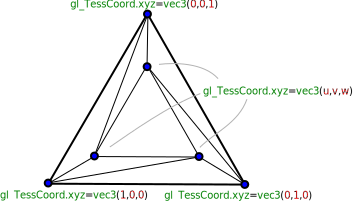
\includegraphics[width=7cm,keepaspectratio]{pics/tessellation/tess_coord.pdf}
	\end{figure}
\end{frame}


\begin{frame}[fragile]
\frametitle{Evaluation Shader - příklad}
	\begin{itemize}
		\item Nateselovaný čtyřúhelník
		\item výpočet pozic vrcholů
	\end{itemize}
	{\scriptsize
	\begin{minted}[frame=lines]{glsl}
#version 430

layout(quads)in;

void main(){
  vec4 A=mix(gl_in[0].gl_Position,gl_in[1].gl_Position,gl_TessCoord.x);
  vec4 B=mix(gl_in[3].gl_Position,gl_in[2].gl_Position,gl_TessCoord.x);
  gl_Position=mix(A,B,gl_TessCoord.y);
}
	\end{minted}
	}
\end{frame}




\begin{frame}[fragile]
  \frametitle{Béziérovy plochy - příklad}
	{\scriptsize
	\begin{minted}[frame=lines]{glsl}
// Vertex shader	
#version 430
void main() {
  gl_Position = mvp*position;
}

// Control shader
#version 430
layout(vertices=16) out;

void main() {
  gl_out[gl_InvocationID].gl_Position =
  gl_in[gl_InvocationID].gl_Position;
  if(gl_InvocationID == 0) {
    gl_TessLevelInner[0] = gl_TessLevelInner[1] = 
    gl_TessLevelOuter[0] = gl_TessLevelOuter[1] =
    gl_TessLevelOuter[2] = gl_TessLevelOuter[3] = 64;
  }
}
	\end{minted}
	}
\end{frame}

\begin{frame}[fragile]
    \frametitle{Béziérovy plochy - příklad}
  	{\scriptsize
		\begin{minted}[frame=lines]{glsl}
// Evaluation shader
#version 430
layout(quads, ccw) in;

vec4 bernstein(float t) {
  return vec4((1-t)*(1-t)*(1-t), 3*t*(1-t)*(1-t), 3*t*t*(1-t), t*t*t);
}

void main() {
  vec4 bu = bernstein(gl_TessCoord.x);
  vec4 bv = bernstein(gl_TessCoord.y);
  vec4 position = vec4(0, 0, 0, 0);
  for(int y = 0; y < 4; ++y){
    for(int x = 0; x < 4; ++x){
      position += bu[x]*bv[y]*gl_in[4*y + x].gl_Position;
    }
  }
  gl_Position = position;
}
  	\end{minted}
		}
\end{frame}

\begin{frame}[fragile]
\frametitle{Komunikace mezi shadery - příklad}
	{\tiny
	\begin{minted}[frame=lines]{glsl}
#version 430

//vertex shader
out vec4 vAttrib;
gl_Position

//control shader
//atribut z vertex shaderu jejich pocet je rizen glPatchParameteri(GL_PATCH_VERTICES,n);
in  vec4 vAttrib[];//atribut z vertex shaderu
gl_in[].gl_Position;//atribut pozice z vertex shaderu
//atribut z control shaderu do evaluation shaderu, pocet je rizen pomoci layout(vertices=n)out;
out vec4 cAttrib[];//atribut pro vrchol z control shaderu do evaluation shaderu
//per patch atribut z control shaderu do evaluation shaderu, pocet je 1
patch out mat4 cM;//atribut pro patch z control shaderu do evaluation shaderu

//evaluation shader
in vec4 cAttrib[];
patch in  mat4 cM;
//atribut z evaluation shaderu do geometry shaderu
out vec3 eNormal;

//geometry shader
//pocet je rizen typem primitiva
in vec3 eNormal[];
	\end{minted}
	}
\end{frame}

\begin{frame}[fragile]
    \frametitle{Příklad - Kružnice vepsaná}
  \begin{columns}[T]
    \begin{column}{.44\textwidth}
	    \begin{figure}[h]
    		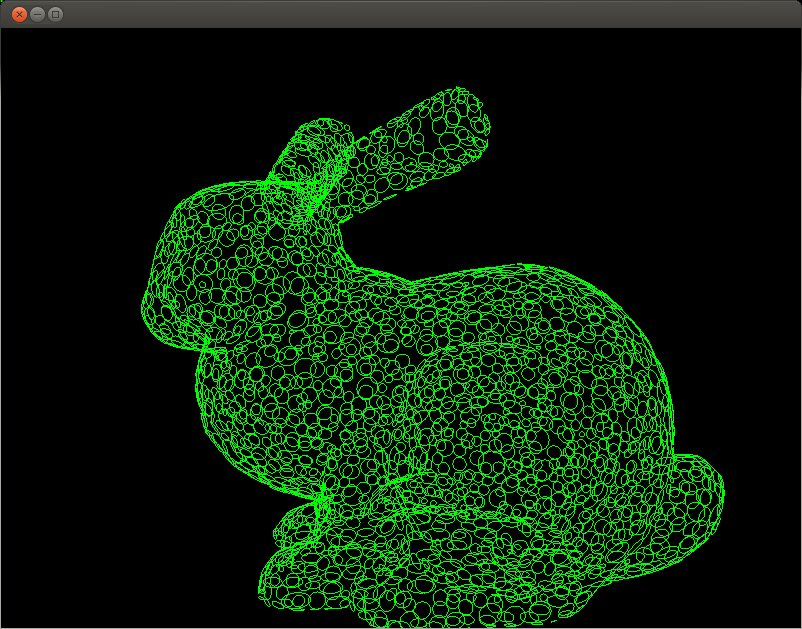
\includegraphics[width=5cm,keepaspectratio]{pics/tessellation/ts_circle}
    	\end{figure}
    \end{column}
    \begin{column}{.48\textwidth}
 	    \begin{figure}[h]
    		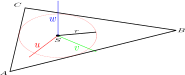
\includegraphics[width=5cm,keepaspectratio]{pics/tessellation/circle.pdf}
    	\end{figure}
{\tiny
$$
K=
\left( 
\begin{array}{cccc} 
1 & 0 & 0 & S_x \\
0 & 1 & 0 & S_y \\
0 & 0 & 1 & S_z \\
0 & 0 & 0 & 1  \\
\end{array}
\right)
\cdot
\left( 
\begin{array}{cccc} 
r & 0 & 0 & 0 \\
0 & r & 0 & 0 \\
0 & 0 & r & 0 \\
0 & 0 & 0 & 1  \\
\end{array}
\right)
\cdot$$
$$
\left( 
\begin{array}{cccc} 
u_x & v_x & w_x & 0 \\
u_y & v_y & w_y & 0 \\
u_z & v_z & w_z & 0 \\
0 & 0 & 0 & 1  \\
\end{array}
\right)
$$
}
    \end{column}
  \end{columns}
\end{frame}

\begin{frame}[fragile]
    \frametitle{Příklad - Kružnice vepsaná}
  \begin{columns}[T]
    \begin{column}{.44\textwidth}
      Control Shader
  	{\tiny
		\begin{minted}[frame=lines]{glsl}
#version 400
layout(vertices=1)out;
patch out mat4 K;
void main(){
  gl_TessLevelOuter[0]=1;
  gl_TessLevelOuter[1]=64;
  gl_TessLevelOuter[2]=1;
  gl_TessLevelOuter[3]=1;
  gl_TessLevelInner[0]=1;
  gl_TessLevelInner[1]=1;
  vec4 TT[3];
  TT[0]=gl_in[0].gl_Position;
  TT[1]=gl_in[1].gl_Position;
  TT[2]=gl_in[2].gl_Position;
  float t01=length((TT[0]-TT[1]).xyz);
  float t02=length((TT[0]-TT[2]).xyz);
  float t12=length((TT[1]-TT[2]).xyz);
  float s=t01+t02+t12;
  float r=sqrt((s/2-t01)*(s/2-t02)*(s/2-t12)*s/2)*2/s;
  t01/=s;
  t02/=s;
  t12/=s;
  vec3 C=TT[0].xyz*t12+TT[1].xyz*t02+TT[2].xyz*t01;
  vec3 x=normalize(TT[0].xyz-C);
  vec3 y=normalize(TT[1].xyz-C);
  vec3 z=normalize(cross(x,y));
  y=normalize(cross(z,x));
  K=mat4(vec4(x,0)*r,vec4(y,0)*r,vec4(z,0)*r,vec4(C,1));
}
  	\end{minted}
		}
    \end{column}
    \begin{column}{.48\textwidth}
      Evaluation Shader
  	{\tiny
		\begin{minted}[frame=lines]{glsl}
#version 400

#define MY_PI 3.14159265359

layout(isolines)in;

uniform mat4 V;
uniform mat4 P;

patch in mat4 K;

void main(){
  float Angle=gl_TessCoord.x*MY_PI*2;
  vec4 PP=vec4(cos(Angle),sin(Angle),0,1);
  gl_Position=P*V*K*PP;
}
  	\end{minted}
		}
    \end{column}
  \end{columns}

\end{frame}


\begin{frame}
\frametitle{Jak moc teselovat?}
	Outer level:
	\begin{itemize}
	\item Strany ploch musí odpovídat (zamezení T-spojů)
	\item Transformovat kontrolní body na obrazovku
	\item Spočítat delků hran
	\item Dělit maximální delkou hrany
	\end{itemize}
	Inner level:
	\begin{itemize}
	\item Z přílušných outer-levelů
	\item průměr, maximum, ...
	\item Korekce podle vnitřních kontrolních bodů
	\end{itemize}
	Ukázka v aplikaci
\end{frame}


\begin{frame}
\frametitle{Beziérová křivka}
$$
{\color{magenta}\vec{P}_{0,1,2,3}(t)}=(1,t^1,t^2,t^3)\cdot
\left(
\begin{array}{cccc}
 1 &  0 &  0 &  0 \\
-3 &  3 &  0 &  0 \\
 3 & -6 &  3 &  0 \\
-1 &  3 & -3 &  1
\end{array}
\right)
\cdot
\left(
\begin{array}{c}
  {\color{green}\vec{P}_{0}} \\
  {\color{green}\vec{P}_{1}} \\
  {\color{green}\vec{P}_{2}} \\
  {\color{green}\vec{P}_{3}} 
\end{array}
\right)
$$
\end{frame}


\begin{frame}
\frametitle{Beziérová křivka}
  \begin{figure}[h]
  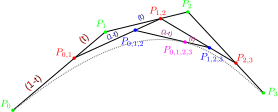
\includegraphics[width=8cm,keepaspectratio]{pics/bezier/bezier}
  \end{figure}
  {\scriptsize
  \[
  \begin{array}{lclcl}
    \color{red}    {\vec{P}_{0,1}    } &=& (1-t)\color{green}{\vec{P}_0      } &+& (t)\color{green}{\vec{P}_1      } \\
    \color{red}    {\vec{P}_{1,2}    } &=& (1-t)\color{green}{\vec{P}_1      } &+& (t)\color{green}{\vec{P}_2      } \\
    \color{red}    {\vec{P}_{2,3}    } &=& (1-t)\color{green}{\vec{P}_2      } &+& (t)\color{green}{\vec{P}_3      } \\
    \color{blue}   {\vec{P}_{0,1,2}  } &=& (1-t)\color{red}  {\vec{P}_{0,1}  } &+& (t)\color{red}  {\vec{P}_{1,2}  } \\
    \color{blue}   {\vec{P}_{1,2,3}  } &=& (1-t)\color{red}  {\vec{P}_{1,2}  } &+& (t)\color{red}  {\vec{P}_{2,3}  } \\
    \color{magenta}{\vec{P}_{0,1,2,3}} &=& (1-t)\color{blue} {\vec{P}_{0,1,2}} &+& (t)\color{blue} {\vec{P}_{1,2,3}} 
  \end{array}
  \]
  }
\end{frame}

\begin{frame}
\frametitle{Beziérová křivka}
  {\tiny
  \[
  \begin{array}{lclcl}
    \color{red}    {\vec{P}_{0,1}    } &=& (1-t)\color{green}{\vec{P}_0      } &+& (t)\color{green}{\vec{P}_1      } \\
    \color{red}    {\vec{P}_{1,2}    } &=& (1-t)\color{green}{\vec{P}_1      } &+& (t)\color{green}{\vec{P}_2      } \\
    \color{red}    {\vec{P}_{2,3}    } &=& (1-t)\color{green}{\vec{P}_2      } &+& (t)\color{green}{\vec{P}_3      } \\
    \color{blue}   {\vec{P}_{0,1,2}  } &=& (1-t)\color{red}  {\vec{P}_{0,1}  } &+& (t)\color{red}  {\vec{P}_{1,2}  } \\
    \color{blue}   {\vec{P}_{1,2,3}  } &=& (1-t)\color{red}  {\vec{P}_{1,2}  } &+& (t)\color{red}  {\vec{P}_{2,3}  } \\
    \color{magenta}{\vec{P}_{0,1,2,3}} &=& (1-t)\color{blue} {\vec{P}_{0,1,2}} &+& (t)\color{blue} {\vec{P}_{1,2,3}} 
  \end{array}
  \]
  }
  {\tiny
  \[
  \begin{array}{lclcl}
    \color{blue}   {\vec{P}_{0,1,2}  } &=& (1-t)((1-t){\color{green}\vec{P}_0} + (t){\color{green}\vec{P}_1}) &+& (t)((1-t){\color{green}\vec{P}_1} + (t){\color{green}\vec{P}_2}) \\
    \color{blue}   {\vec{P}_{1,2,3}  } &=& (1-t)((1-t){\color{green}\vec{P}_1} + (t){\color{green}\vec{P}_2}) &+& (t)((1-t){\color{green}\vec{P}_2} + (t){\color{green}\vec{P}_3}) \\
    \color{magenta}{\vec{P}_{0,1,2,3}} &=& (1-t)\color{blue} {\vec{P}_{0,1,2}} &+& (t)\color{blue} {\vec{P}_{1,2,3}} 
  \end{array}
  \]
  }
  {\tiny
  \[
  \begin{array}{lclccrc}
    \color{magenta}{\vec{P}_{0,1,2,3}} &=& (1-t)&(1-t)&(1-t)&{\color{green}\vec{P}_0} &+ \\
                                       & & (1-t)&(1-t)&(  t)&{\color{green}\vec{P}_1} &+ \\
                                       & & (1-t)&(  t)&(1-t)&{\color{green}\vec{P}_1} &+ \\
                                       & & (1-t)&(  t)&(  t)&{\color{green}\vec{P}_2} &+ \\
                                       & & (  t)&(1-t)&(1-t)&{\color{green}\vec{P}_1} &+ \\
                                       & & (  t)&(1-t)&(  t)&{\color{green}\vec{P}_2} &+ \\
                                       & & (  t)&(  t)&(1-t)&{\color{green}\vec{P}_2} &+ \\
                                       & & (  t)&(  t)&(  t)&{\color{green}\vec{P}_3} &
  \end{array}
  \]
  }
  {\tiny
  \[
  \begin{array}{lclccrc}
    \color{magenta}{\vec{P}_{0,1,2,3}} &=& (1-t)&(1-t)&(1-t)&{\color{green}\vec{P}_0} &+ \\
                                       & & 3(1-t)&(1-t)&(  t)&{\color{green}\vec{P}_1} &+ \\
                                       & & 3(1-t)&(  t)&(  t)&{\color{green}\vec{P}_2} &+ \\
                                       & & (  t)&(  t)&(  t)&{\color{green}\vec{P}_3} &
  \end{array}
  \]
  }

\end{frame}

\begin{frame}
\frametitle{Beziérová křivka}
  {\tiny
  \[
  \begin{array}{lclccrc}
    \color{magenta}{\vec{P}_{0,1,2,3}} &=& (1-t)&(1-t)&(1-t)&{\color{green}\vec{P}_0} &+ \\
                                       & & 3(1-t)&(1-t)&(  t)&{\color{green}\vec{P}_1} &+ \\
                                       & & 3(1-t)&(  t)&(  t)&{\color{green}\vec{P}_2} &+ \\
                                       & & (  t)&(  t)&(  t)&{\color{green}\vec{P}_3} &
  \end{array}
  \]
  }
  {\tiny
  \[
  \begin{array}{lclrc}
    \color{magenta}{\vec{P}_{0,1,2,3}} &=& (1-t)^3&{\color{green}\vec{P}_0} &+ \\
                                       & & 3(1-t)^2(t)&{\color{green}\vec{P}_1} &+ \\
                                       & & 3(1-t)(t)^2&{\color{green}\vec{P}_2} &+ \\
                                       & & (t)^3&{\color{green}\vec{P}_3} &
  \end{array}
  \]
  }
  {\tiny
  \[
  \begin{array}{lclrc}
    \color{magenta}{\vec{P}_{0,1,2,3}} &=& \dbinom{3}{0}(1-t)^{3-0}(t)^{0}&{\color{green}\vec{P}_0} &+ \\
                                       & & \dbinom{3}{1}(1-t)^{3-1}(t)^{1}&{\color{green}\vec{P}_1} &+ \\
                                       & & \dbinom{3}{2}(1-t)^{3-2}(t)^{2}&{\color{green}\vec{P}_2} &+ \\
                                       & & \dbinom{3}{3}(1-t)^{3-3}(t)^{3}&{\color{green}\vec{P}_3} &
  \end{array}
  \]
  }
  {\tiny
  $$
  {\color{magenta}\vec{P}_{0,1,2,3}(t)} = \sum\limits_{i=0}^{i \leq 3}\dbinom{3}{i}(1-t)^{3-i}(t)^{i}{\color{green}\vec{P}_i} 
  $$
  }
  {\tiny
  $$
  {\color{magenta}\vec{P}(t)} = \sum\limits_{i=0}^{i \leq n-1}\dbinom{n-1}{i}(1-t)^{n-1-i}(t)^{i}{\color{green}\vec{P}_i} 
  $$
  }


\end{frame}

\begin{frame}
\frametitle{Beziérová křivka}
  {\tiny
  \[
  \begin{array}{lclrc}
    \color{magenta}{\vec{P}_{0,1,2,3}(t)} &=& (1-t)^3&{\color{green}\vec{P}_0} &+ \\
                                       & & 3(1-t)^2(t)&{\color{green}\vec{P}_1} &+ \\
                                       & & 3(1-t)(t)^2&{\color{green}\vec{P}_2} &+ \\
                                       & & (t)^3&{\color{green}\vec{P}_3} &
  \end{array}
  \]
  }
  {\tiny
  \[
  \begin{array}{lclrc}
    \color{magenta}{\vec{P}_{0,1,2,3}(t)} &=& (1-3t+3t^2-t^3)&{\color{green}\vec{P}_0} &+ \\
                                       & & (3t-6t^2+3t^3)&{\color{green}\vec{P}_1} &+ \\
                                       & & (3t^2-3t^3)&{\color{green}\vec{P}_2} &+ \\
                                       & & (t^3)&{\color{green}\vec{P}_3} &
  \end{array}
  \]
  }
  {\tiny
$$
{\color{magenta}\vec{P}_{0,1,2,3}(t)}=(1,t^1,t^2,t^3)\cdot
\left(
\begin{array}{cccc}
 1 &  0 &  0 &  0 \\
-3 &  3 &  0 &  0 \\
 3 & -6 &  3 &  0 \\
-1 &  3 & -3 &  1
\end{array}
\right)
\cdot
\left(
\begin{array}{c}
  {\color{green}\vec{P}_{0}} \\
  {\color{green}\vec{P}_{1}} \\
  {\color{green}\vec{P}_{2}} \\
  {\color{green}\vec{P}_{3}} 
\end{array}
\right)
$$
  }
\end{frame}

\begin{frame}
\frametitle{Beziérová plocha}
  \begin{figure}[h]
  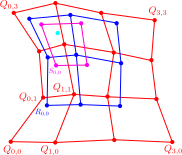
\includegraphics[width=5cm,keepaspectratio]{pics/bezier/bezier3}
  \end{figure}
  {\tiny
  \[
  \begin{array}{ccclllllll}
    {\color{blue}R_{0,0}} &=& (1-l)(1-t){\color{red}Q_{0,0}} &+& (1-l)(t){\color{red}Q_{1,0}}   &+& (l)(1-t){\color{red}Q_{0,1}}   &+& (l)(t){\color{red}Q_{1,1}} \\
    {\color{blue}R_{1,0}} &=& (1-l)(1-t){\color{red}Q_{1,0}} &+& (1-l)(t){\color{red}Q_{2,0}}   &+& (l)(1-t){\color{red}Q_{1,1}}   &+& (l)(t){\color{red}Q_{2,1}} \\
    {\color{blue}R_{2,0}} &=& (1-l)(1-t){\color{red}Q_{2,0}} &+& (1-l)(t){\color{red}Q_{3,0}}   &+& (l)(1-t){\color{red}Q_{2,1}}   &+& (l)(t){\color{red}Q_{3,1}} \\
                         &&&&\vdots &&&& \\
    {\color{blue}R_{i,k}} &=& (1-l)(1-t){\color{red}Q_{i,k}} &+& (1-l)(t){\color{red}Q_{i+1,k}} &+& (l)(1-t){\color{red}Q_{i,k+1}} &+& (l)(t){\color{red}Q_{i+1,k+1}} \\
  \end{array}
  \]
  }
  {\tiny
  \[
  \begin{array}{ccclllllll}
    {\color{blue}R_{i,k}} &=& (1-l)(1-t){\color{red}Q_{i,k}} &+& (1-l)(t){\color{red}Q_{i+1,k}} &+& (l)(1-t){\color{red}Q_{i,k+1}} &+& (l)(t){\color{red}Q_{i+1,k+1}}        \\
    {\color{magenta}S_{i,k}} &=& (1-l)(1-t){\color{blue}R_{i,k}} &+& (1-l)(t){\color{blue}R_{i+1,k}} &+& (l)(1-t){\color{blue}R_{i,k+1}} &+& (l)(t){\color{blue}R_{i+1,k+1}} \\
    {\color{cyan}X_{i,k}} &=& (1-l)(1-t){\color{magenta}S_{i,k}} &+& (1-l)(t){\color{magenta}S_{i+1,k}} &+& (l)(1-t){\color{magenta}S_{i,k+1}} &+& (l)(t){\color{magenta}S_{i+1,k+1}}
  \end{array}
  \]
  }
\end{frame}



\begin{frame}
\frametitle{Catmullrom}
  \begin{figure}[h]
  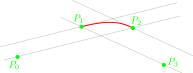
\includegraphics[width=5cm,keepaspectratio]{pics/catmullrom/catmullrom}
  \end{figure}
  {\scriptsize
    $$
v(t)=(1,t^1,t^2,t^3)\cdot
\frac{1}{2}\cdot
\left(
\begin{array}{cccc}
 0 &  2 &  0 &  0 \\
-1 &  0 &  1 &  0 \\
 2 & -5 &  4 & -1 \\
-1 &  3 & -3 &  1
\end{array}
\right)
\cdot
\left(
\begin{array}{c}
  {\color{green}P_{0}} \\
  {\color{green}P_{1}} \\
  {\color{green}P_{2}} \\
  {\color{green}P_{3}} 
\end{array}
\right)
$$
  }
\end{frame}

\begin{frame}
\frametitle{Catmullrom}
  \begin{figure}[h]
  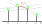
\includegraphics[width=5cm,keepaspectratio]{pics/catmullrom/catmullrom2}
  \end{figure}
  {\scriptsize
    \[
    \begin{array}{ccc}
      f(0) &=& {\color{green}P_1} \\
      f(1) &=& {\color{green}P_2} \\
     f'(0) &=& \frac{{\color{green}P_2}-{\color{green}P_0}}{2} \\
     f'(1) &=& \frac{{\color{green}P_3}-{\color{green}P_1}}{2} \\
      f(t) &=& \sum\limits_{i=0}^{i \leq 3}(a_i+b_it+c_it^2+d_it^3){\color{green}P_i}
    \end{array}
    \]
  }
\end{frame}


\begin{frame}
    \frametitle{Béziérovy plochy}

    
\includegraphics[height=.3\textheight]{pics/tessellationBezier/bezier.eps}

    \begin{eqnarray*}
        B_{n,k}(t) &=& {n\choose k}t^k\left(1-t\right)^{\left(n-k\right)}\\
        P(t)      &=& \left[\left(B_{n,0}(t),\ldots,B_{n,n}(t)\right)\left(
            \begin{array}{ccc}
                x_0 & y_0 & \ldots\\
                x_1 & y_1 & \ldots\\
                &\ldots&
            \end{array}\right)\right]\\
        P_{\{x,y,z\}}(u,v) &=& \left[\left(B_{n,0}(u),\ldots,B_{n,n}(u)\right)K_{\{x,y,z\}}\left(
            \begin{array}{c}B_{n,0}(v)\\\ldots\\B_{n,n}(v)\end{array}\right)\right]
    \end{eqnarray*}
\end{frame}

\begin{frame}
    \frametitle{Racionální béziérky}

    Kontrolní body mají i váhu :
    \begin{equation*}
        P(t) = \frac{ \sum_{i=0}^n B_{i,n}(t) \mathbf{P_i w_i} }{ \sum_{i=0}^n B_{i,n}(t) \mathbf{w_i} }
    \end{equation*}
    \pause\vfill
    \begin{itemize}
        \item Váha táhne plochu blíž k bodu.
        \item Kontrolní body s vahou jsou homogenní souøadnice.
        \item Jdou bez problémù i promítnout.
    \end{itemize}
\end{frame}    

\begin{frame}[fragile]
\frametitle{Vertex Shader}
	{\scriptsize
	\begin{minted}[frame=lines]{glsl}
#version 410

uniform mat4 mvp;

layout(location=0) in vec4 position;

void main()
{
    gl_Position = mvp*position;
}
	\end{minted}
	}
\end{frame}

\begin{frame}[fragile]
\frametitle{Fragment Shader}
	{\scriptsize
	\begin{minted}[frame=lines]{glsl}
#version 410

flat in vec4 color;

out vec4 output;

void main()
{
    output = color;
}
	\end{minted}
	}
\end{frame}

\begin{frame}[fragile]
\frametitle{Control Shader}
	{\scriptsize
	\begin{minted}[frame=lines]{glsl}
#version 410

layout(vertices=16) out;

void main()
{
    gl_out[gl_InvocationID].gl_Positiono
        = gl_in[gl_InvocationID].gl_Position;
    if(gl_InvocationID == 0)
    {
        gl_TessLevelInner[0] = 8;
        gl_TessLevelInner[1] = 8;
        gl_TessLevelOuter[0] = 64;
        gl_TessLevelOuter[1] = 64;
        gl_TessLevelOuter[2] = 64;
        gl_TessLevelOuter[3] = 64;
    }
}
	\end{minted}
	}
\end{frame}

\begin{frame}[fragile]
\frametitle{Evaluation Shader}
	{\scriptsize
	\begin{minted}[frame=lines]{glsl}
#version 410
layout(quads, equal_spacing, ccw) in;
flat out vec4 color;
vec4 bernstein(float t)
{
  return vec4((1-t)*(1-t)*(1-t),3*t*(1-t)*(1-t),3*t*t*(1-t), t*t*t);
}
void main()
{
  vec4 bu = bernstein(gl_TessCoord.x);
  vec4 bv = bernstein(gl_TessCoord.y);
  vec4 position = vec4(0,0,0,0);
  for(int y = 0; y < 4; ++y)
    for(int x = 0; x < 4; ++x)
      position += bu[x]*bv[y]*gl_in[4*y+x].gl_Position;
  gl_Position = position;
  color = vec4(gl_TessCoord.xy,0,1);
}
	\end{minted}
	}
\end{frame}


\begin{frame}
  \frametitle{References}
  \begin{itemize}
    \item \url{http://www.opengl.org/sdk/docs/}
    \item \url{http://www.opengl.org/documentation/glsl/}
    \item \url{http://www.opengl.org/registry/}
  \end{itemize}
\end{frame}



\bluepage{Thank you for your attention! \vspace{10 mm} Questions?}

\end{document}
